% Chapter X

\chapter{Généralité} % Chapter title


\label{ch:02-01} % For referencing the chapter elsewhere, use \autoref{ch:name} 

%----------------------------------------------------------------------------------------

% \section{}

La mucoviscidose est une maladie à transmission autosomique et récessive multiviscérale, autrement dit, c’est une maladie qui peut toucher de nombreux organes et seul les personnes ayant hérité de deux mutations, provenant l’un du père et l’autre de leur mère, sont atteintes. Elle touche essentiellement les personnes d’origine caucasienne et est très rarement retrouvé en Asie et en Afrique. La mucoviscidose est causé par des mutations dans un gène identifié en 1989 (Riordan et al. 1989)\cite{riordan_identification_1989} et localisé sur le bras long (appelé q) du chromosome 7 à la position 31.2 (7q31.2). Ce gène appelé CFTR (Cystic fibrosis transmembrane conductance regulator) code pour une glycoprotéine membranaire de même nom retrouvée au pôle apical de la majorité des cellules épithéliale. 
C’est en 1938 à la suite d’autopsie d’enfants souffrant de malnutrition que pour la première fois la distinction fut établie entre la maladie cœliaque et la mucoviscidose défini à l’époque par le terme de « fibrose cystique du pancréas ». Elle fut décrite comme une maladie caractérisée par une mauvaise absorption des graisses et protéines, une stéatorrhée (quantité élevée de lipides dans les selles), un retard de croissance et des infections pulmonaires (ANDERSEN DH 1938)\cite{andersen_dh_cystic_1938}. Ce n’est qu’en 1943 qu’elle fut renommé « mucoviscidose » afin de rendre compte de l’état visqueux du mucus généralisé à plusieurs organes autre que le pancréas (Farber 1943)\cite{farber_pancreatic_1943}. En 1948 lors de la vague de chaleur à New York un jeune pédiatre, Paul di Sant'Agnese, constata que beaucoup de nourrissons atteint de mucoviscidose présentaient une prostration due à la chaleur. Il émit l’hypothèse d’un problème de sudation et démontra un excès de sodium et de chlorure cinq fois plus important dans la sueur des patients atteints de mucoviscidose, qui persistait même après la vague de chaleur(Di Sant’agnese et al. 1953)\cite{di_santagnese_abnormal_1953}. C’est grâce à cette découverte que sera mis au point un peu plus tard le test de la sueur toujours utilisé de nos jours afin de diagnostiquer les patients (Gibson and Cooke 1959)\cite{gibson_test_1959}.
Selon le registre français de la mucoviscidose en 2014 on comptait un peu plus de 6000 patients recensés. Ce nombre, en constante progression depuis le début du recensement en 1992, compte pour la deuxième fois consécutive, même si la population reste jeune avec un âge moyen d’environ 20 ans, plus d’adultes que d’enfants. (Figure \ref{patient} et Figure \ref{evolutionpatient})
\begin{center}
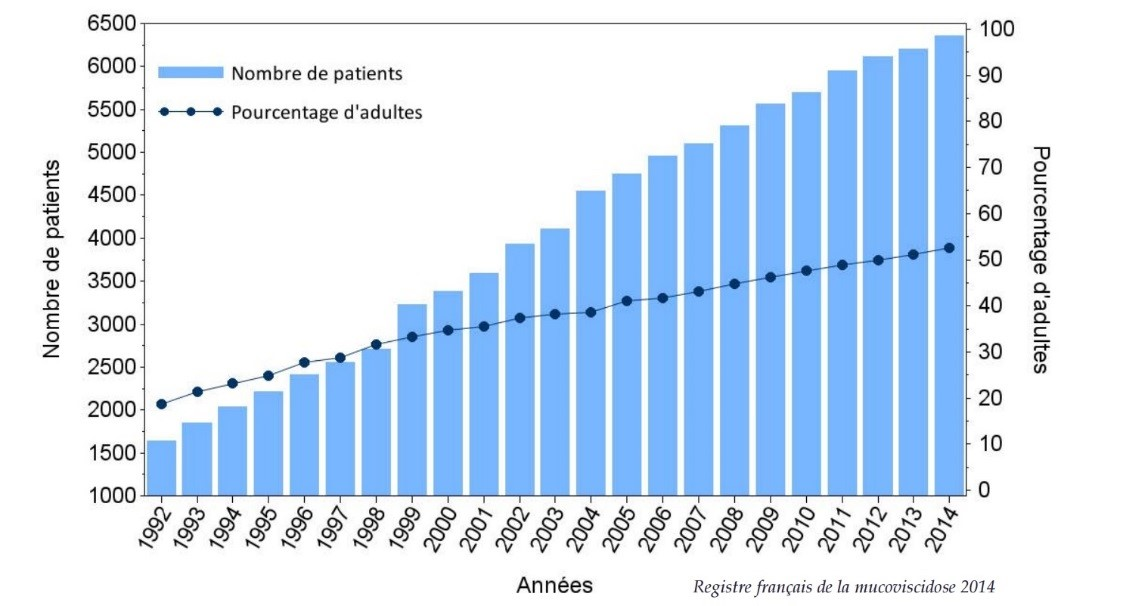
\includegraphics[scale=1]{gfx/patient.jpg} 
\captionsetup{type=figure}
\captionof{figure}{Nombre de patients vus dans l'année et pourcentage d'adultes (registre français de la mucoviscidose)}
       \label{patient}
\end{center}
\begin{center}
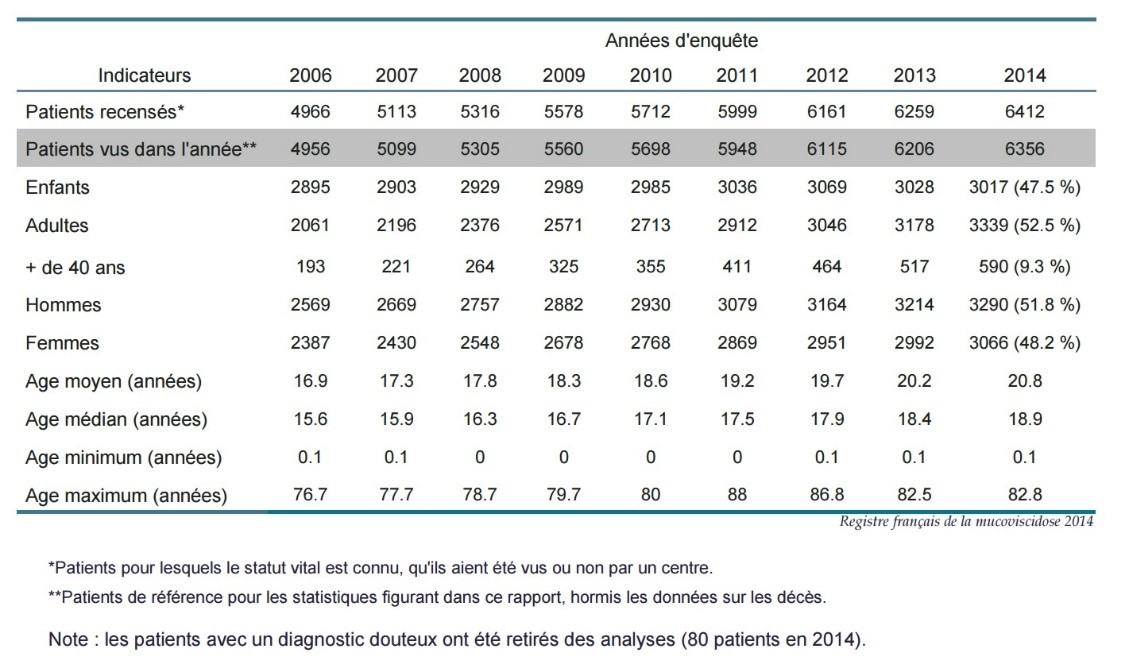
\includegraphics[scale=1]{gfx/evolutionpatient.jpg} 
\captionsetup{type=figure}
\captionof{figure}{Evolution annuelle des principaux indicateurs (registre français de la mucoviscidose)}
       \label{evolutionpatient}
\end{center}
	
%------------------------------------------------

% \subsection{Subsection Title}

% Content